\section{Results and Discussion}



Establishing X-ray tomography as a valid approach: references for absorption correction calculations

3D plots of finding the most optimal ACs for crystal and liquor using AnACor's AC values at 0.5 acceptance percentage as the reference

This validation experiment ultimately took AC values calculated by AnACor in its pre-processing stage as a reference to run the post-processing of AnACor on a combination of AC of crystal and liquor varied in several increments from the reference. The aim of this was a check of AnACor's accuracy in determining the optimal AC that maximise the $I/ \sigma$ results while minimising the $R_{merge}$ factor.

In the interest of time, this validation check was not applied to the crystals investigated in the remainder of this paper. The scripts and methods for this validation have been completed so that it can be applied to future tomography data being processed at I23.

 

\subsection{Comparison of an empirical, analytical, and coupled approach to absorption corrections}

Merging statistics and anomalous peak heights \cite{LuSubmitted}

\begin{figure}[h]
    \centering
    \begin{tabular}{cc}
    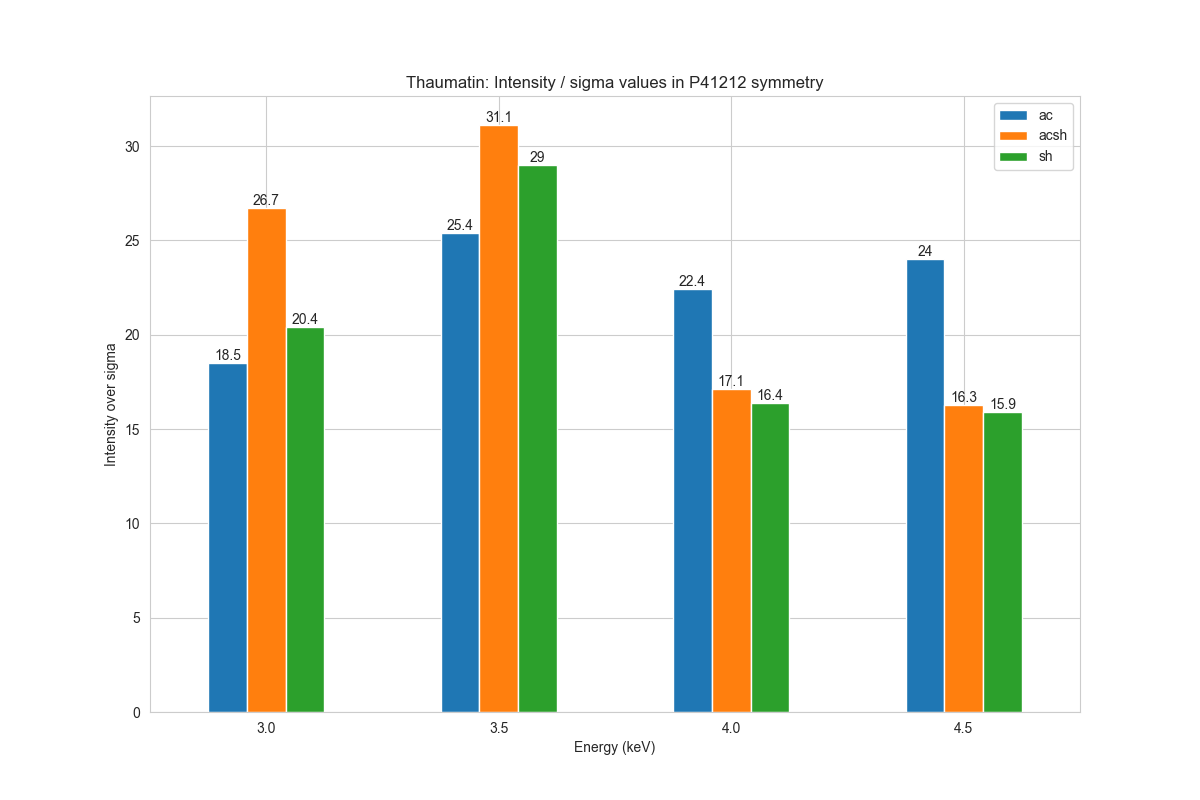
\includegraphics[width = 0.5\textwidth]{plots/Experiment 1/thaum_1/I_over_sigma.png} & 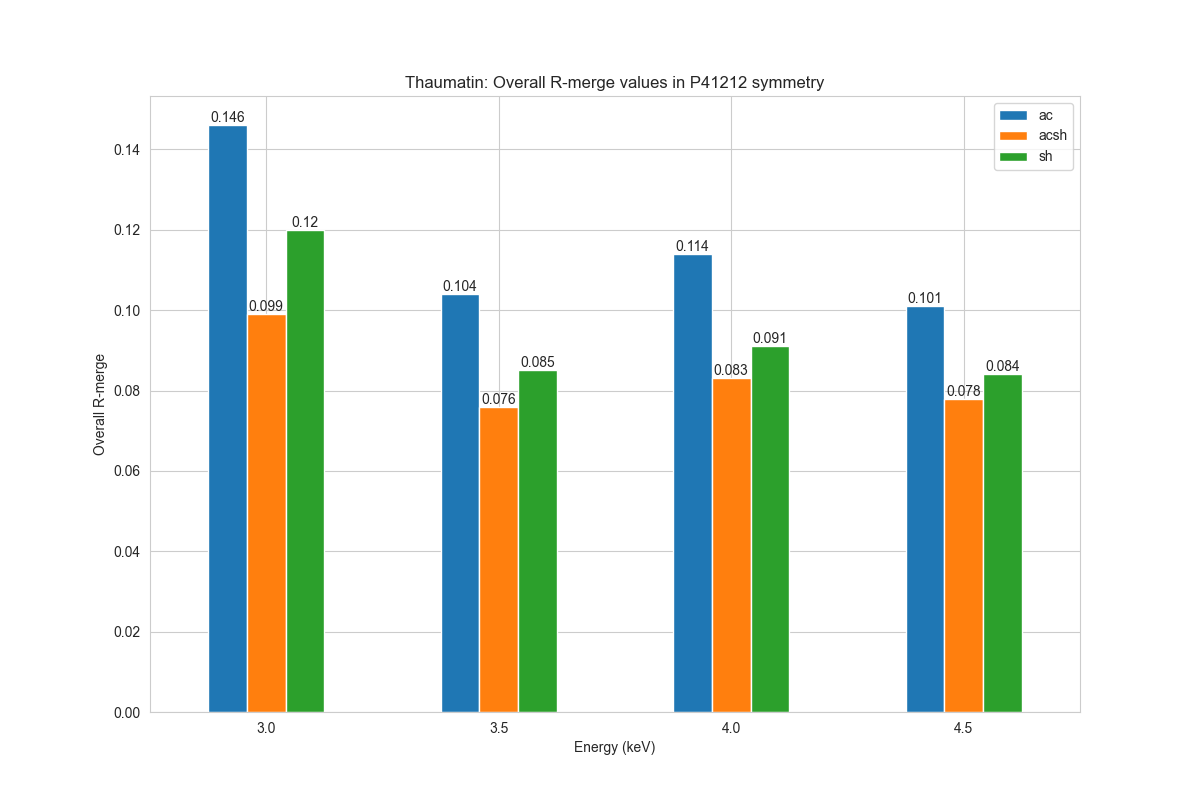
\includegraphics[width = 0.5\textwidth]{plots/Experiment 1/thaum_1/rmerges.png}
    \end{tabular}
    \caption{Caption}
    \label{fig:thaum1_Isig}
\end{figure}

In the interest of observing the effects of high absorption, subsequent crystal samples were largely collected at 3.0 and 3.5 keV, the lowest energies accessible to I23.

Subsequent tomography experiments were performed on two protein crystals of thermolysin. The first crystal, referred to as \ac{t1}, was collected at three energies: 3.0, 3.5, and 3.8 keV, with five to eight datasets at each energy of varying orientations of $\kappa$ and $\phi$, as listed in cref table. The subsequent thermolysin crystal was collected only at 3.0 and 3.5 keV with four and five datasets respectively of varying orientations, also seen in cref table.

Thermolysin belongs to the symmetry space group \textit{P6122}. While processing in P6122 is therefore the .

Results from \ac{t2} overwhelmingly show that \ac{acsh} is the dominating correction method, with intensities peaking and the R factors dipping across every dataset.

The results of 

\begin{figure}[h]
    \centering
    \begin{tabular}{cc}
    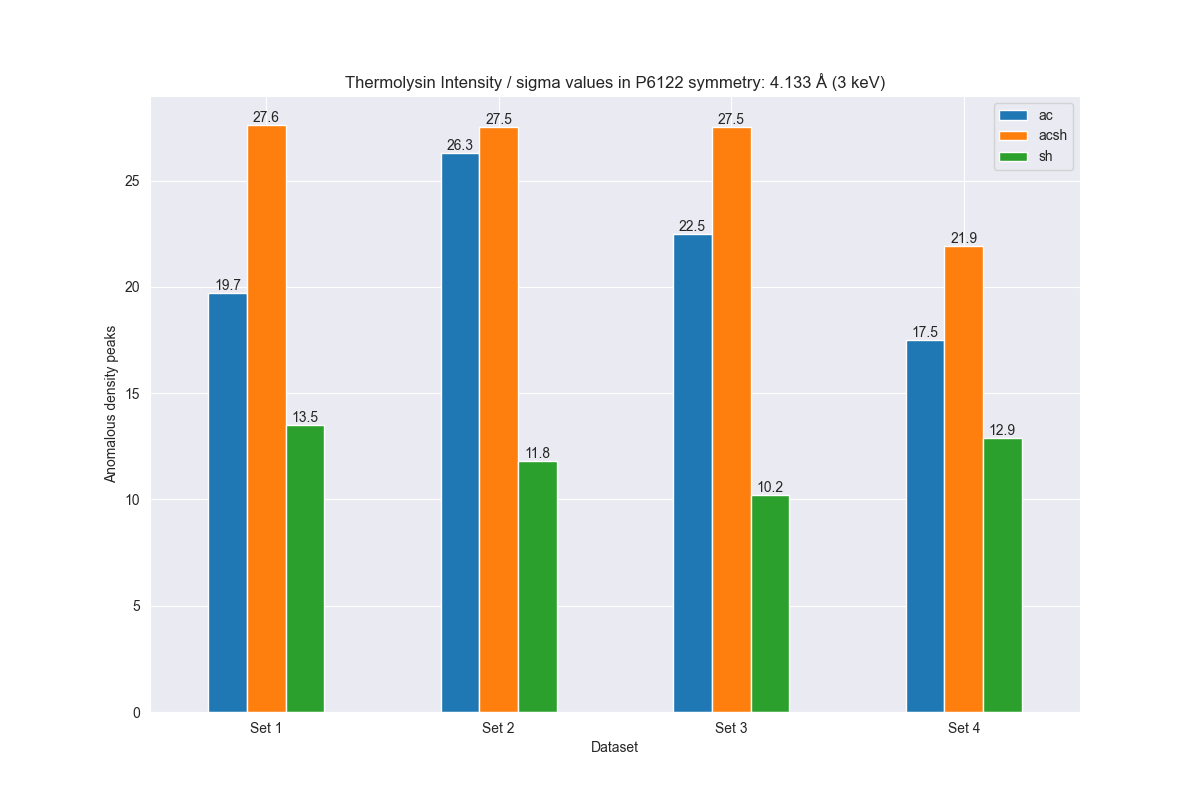
\includegraphics[width = 0.5\textwidth]{plots/Experiment 1/tlys_2 P6122/3p0_I_over_sigma.png} & 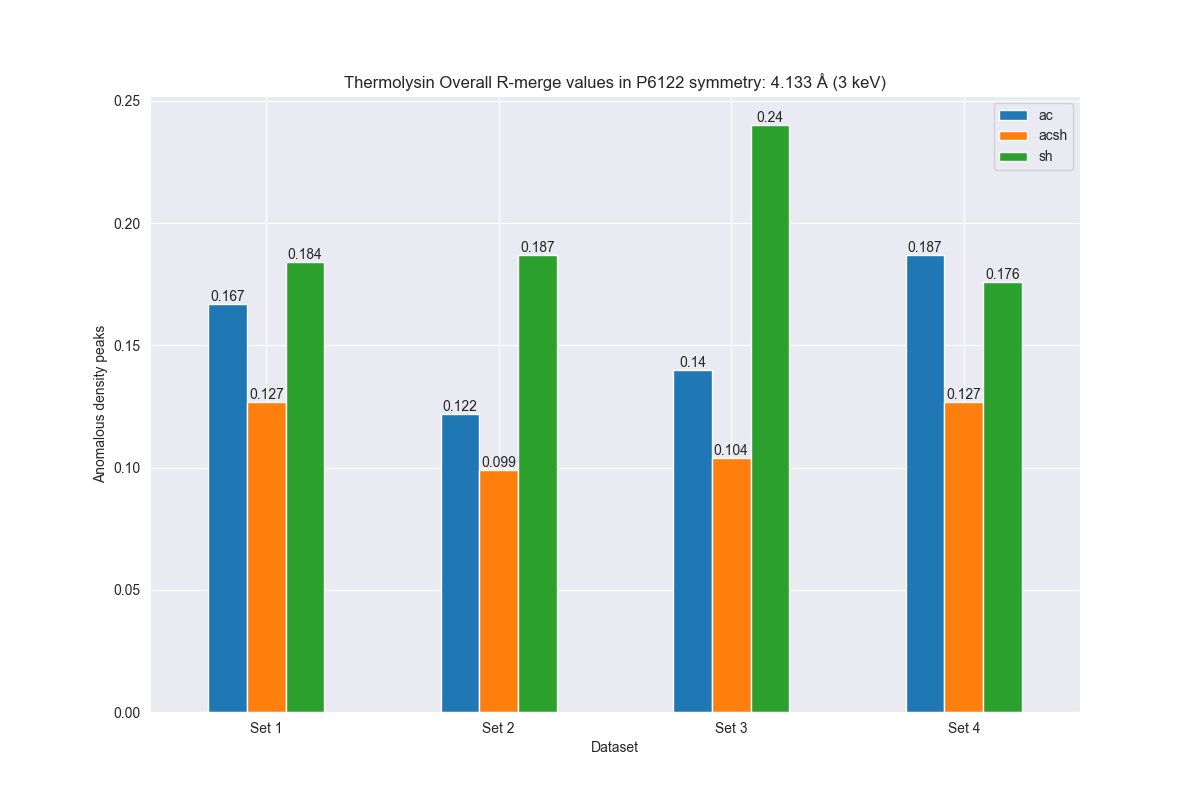
\includegraphics[width = 0.5\textwidth]{plots/Experiment 1/tlys_2 P6122/3p0_rmerges.png}
    \end{tabular}
    \caption{Caption}
    \label{fig:tlys_2_p6}
\end{figure}

\subsection{Absorption corrections on laser-shaped samples}

\begin{figure}[h]
    \centering
    \begin{tabular}{cc}
    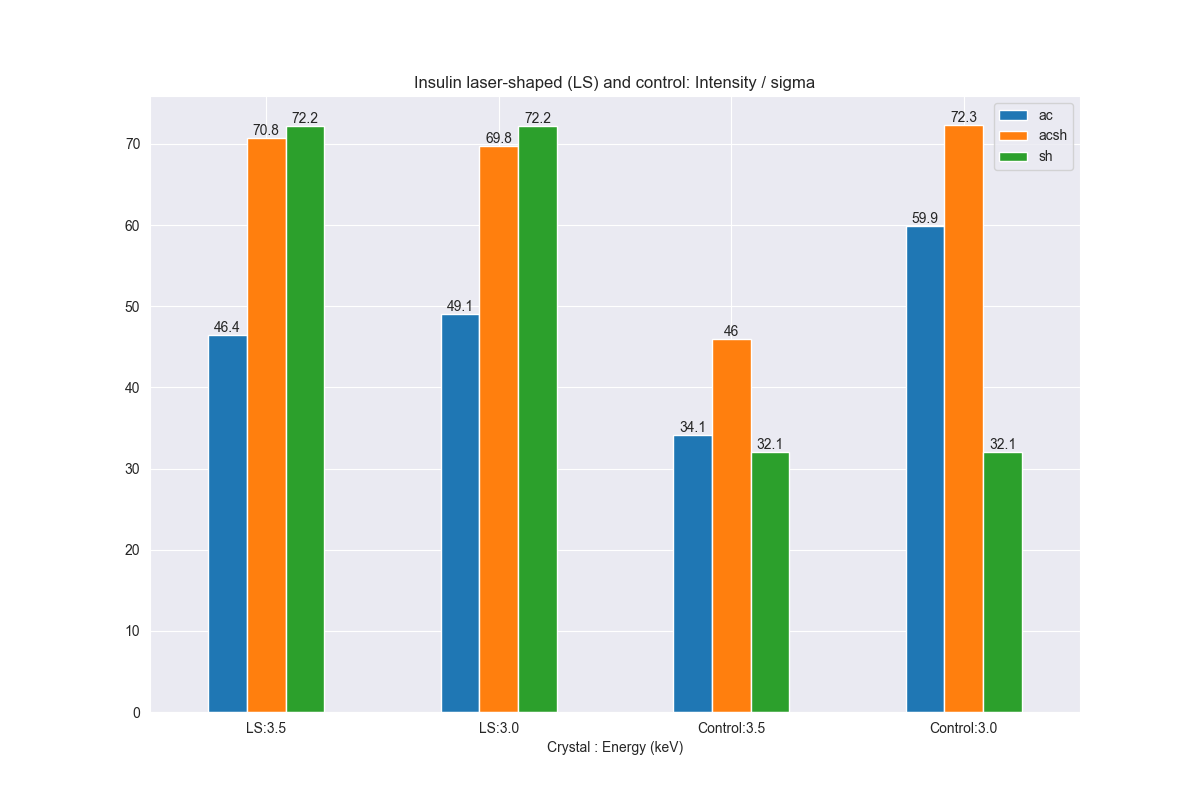
\includegraphics[width = 0.5\textwidth]{plots/Experiment 2 LS/ins_I_over_sigma.png} & 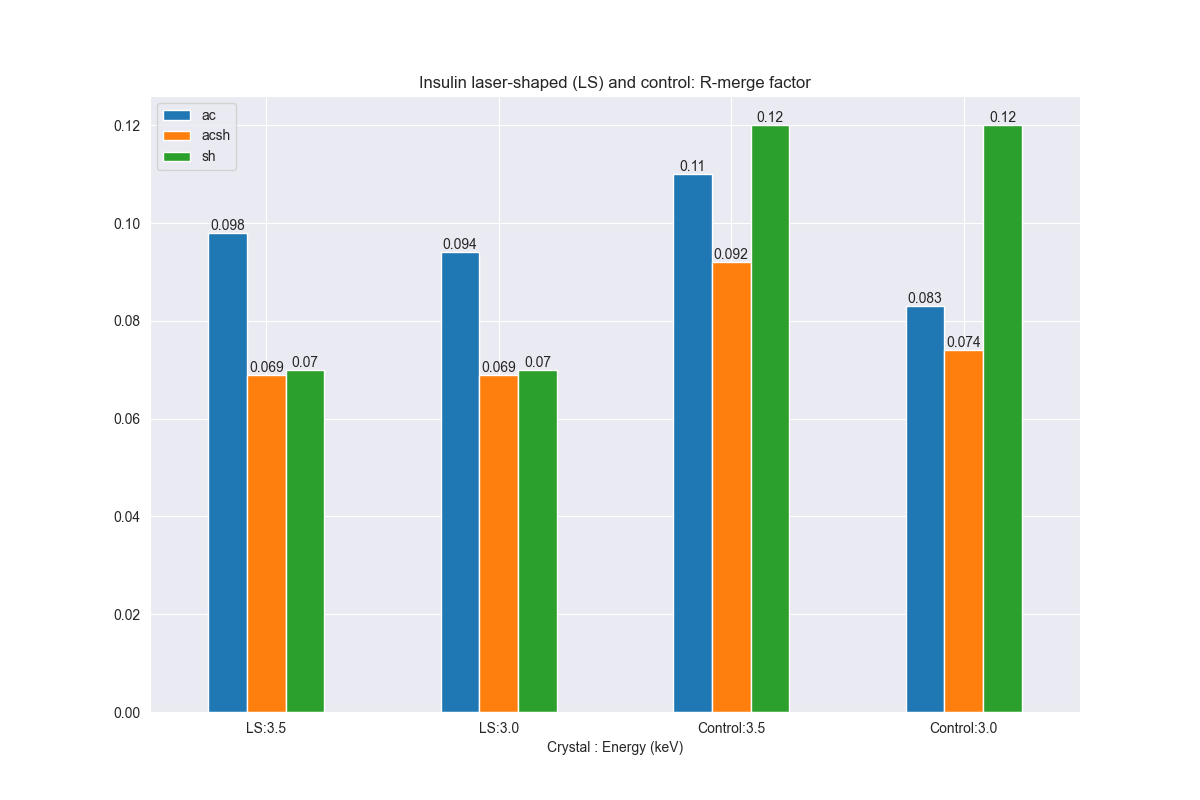
\includegraphics[width = 0.5\textwidth]{plots/Experiment 2 LS/ins_rmerges.png}
    \end{tabular}
    \caption{Caption}
    \label{fig:insulin}
\end{figure}


Testing tomo on lysosyme to try to detect sodium anomalous signal

Mention LASER-shaping already worked on identifying magnesium in topoisomerase crystals. Hypothesis: tomography can do the same

\subsection{Tomography-constructed analytical models in ion identification via $f"$-refinement}

As of this year, I23 has established a new method of ion identification using anomalous scattering known as f" refinement. This protocol uses a programme known as Phenix which has a feature for estimating the f' and f" values of a given element based on the (mtz and pdb) of the collected crystal data. The f"-refinement is becoming a routinely-used feature of ion identification due to the long wavelength capabilities of the beamline. 

test

\subsection{Errors and Improvement}

Faults in anacor thresholding, particularly at processing datasets collected at multiple energies

segmentation at high contrast

There are several challenges associated with the segmentation of X-ray data of protein crystals.